\section{Loss function} \label{sec:loss-fn}
Used to quantify the difference between prediction and actual value in
a way that the minimization of the value of this function is an
optimization problem that is convenient to tackle.
Loss functions are also known as \emph{error functions}.

A sample loss function using squared errors:

\begin{mathpar}
  L(\hat{y}, y) = \frac{1}{2} (\hat{y} - y)^{2}
\end{mathpar}

\section{Sigmoid function} \label{sec:sigmoid-fn}
aka logistic function.

\begin{mathpar}
  f(x) = \frac{1}{1+e^{-x}}
\end{mathpar}

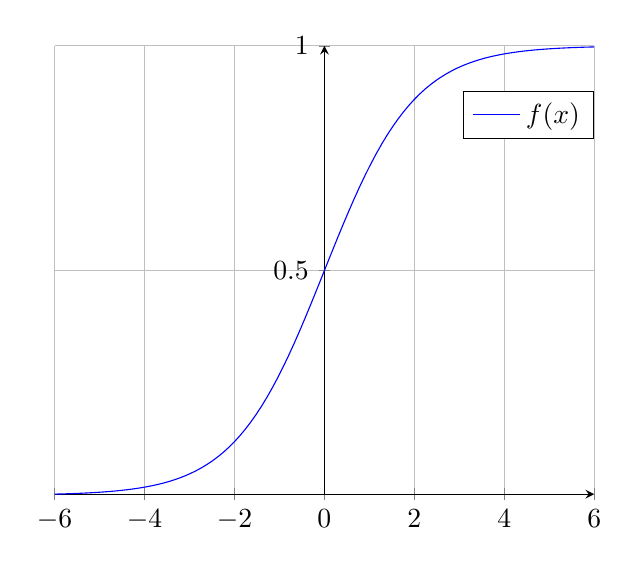
\begin{tikzpicture}[%
  declare function={%
    sigma(\x)=1/(1+exp(-\x));
    }%
]
% https://tex.stackexchange.com/questions/497949/drawing-a-sigmoid-function-and-its-derivative-in-tikz
\begin{axis}%
[
  grid=major,     
  xmin=-6,
  xmax=6,
  axis x line=bottom,
  ytick={0,.5,1},
  ymax=1,
  axis y line=middle,
  samples=100,
  domain=-6:6,
  legend style={at={(1,0.9)}}     
]
    \addplot[blue,mark=none]   (x,{sigma(x)});
    \legend{$f(x)$}
\end{axis}
\end{tikzpicture}

\begin{itemize} 
  \item Grows gently, from \emph{almost} $0$
  \item Midpoint $f(0) = 0.5$ 
  \item $y \in (0, 1)$
  \item Decays gently, \emph{towards} $1$
  \item $f(x)$ is $1$ for large positive $x$ as $e^{-x}$ tends to $0$
  \item $f(x)$ is $0$ for large negative $x$ as $e^{-x}$ gets bigger
\end{itemize} 

\section{ReLu function} \label{sec:relu-fn}

\begin{mathpar}
  f(x) = max(0, x) =
\left\{
    \begin{aligned}
         & x \quad & x > 0 \\
         & 0 \quad & x \leq 0 \\ 
    \end{aligned}
\right.
\end{mathpar}

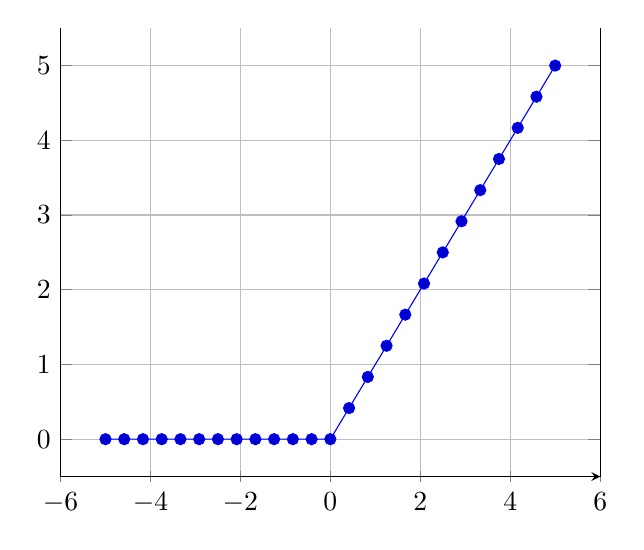
\begin{tikzpicture}
 % https://tex.stackexchange.com/questions/334588/how-to-draw-relu-function
\begin{axis}[
  grid=major,     
  xmin=-6,
  xmax=6,
  axis x line=bottom,
  %ytick={0,.5,1},
  %ymax=1,
  %domain=-3:5,
  legend style={at={(1,0.9)}}     
]
  \addplot {(x>=0)*x};
\end{axis}
\end{tikzpicture}

\begin{itemize} 
  \item Rectified Linear Unit
  \item Zero for negative values, id for others
  \item Essentially cuts off values less than zero
\end{itemize} 
